%!TEX program = xelatex

\documentclass[11pt]{article}
\usepackage{geometry}
\usepackage{tcolorbox}
\usepackage{hyperref}
\usepackage{microtype}
\usepackage{rotating}
\usepackage[backend=biber,sorting=none,style=apa]{biblatex}
\addbibresource{library.bib}
\geometry{
    a4paper,
    total={170mm,257mm},
    left=20mm,
    top=20mm,
}
\setlength{\parskip}{5pt}
\setlength\parindent{0pt}
\usepackage{graphicx}
\usepackage{booktabs}
\usepackage{subcaption}
\usepackage{amsmath}
\usepackage{amsfonts}
\usepackage{amssymb}
\usepackage{lscape}
\usepackage{psfrag}
\usepackage{hyperref}
\hypersetup{
  colorlinks = false,
  urlcolor   = blue,
  linkcolor  = blue,
  citecolor  = red
}
\usepackage{verbatim}
\usepackage{textcomp}
\usepackage{multirow}
\usepackage{rotating}
\usepackage{adjustbox}
\usepackage{tikz}
\usepackage[english]{babel}
\usepackage{appendix}
\usepackage{parskip}
\usepackage{placeins}
\usepackage[tableposition=top]{caption}
\captionsetup{skip=0pt}

\usepackage{amsmath}
\usepackage{fontspec}
\usepackage[charter]{newtxmath}

\setmainfont{XCharter}
\newfontfamily{\XCharterLF}{XCharter}[NFSSFamily=xcharterlf]

\DeclareSymbolFont{operators}{TU}{xcharterlf}{m}{n}

\usepackage{listings}
\lstset{
  language=R,
  basicstyle=\footnotesize,
  numbers=left,
  numberstyle=\tiny,
  numbersep=5pt,
  showstringspaces=false,
  frame=single
} 

\sloppy
\widowpenalty=10000
\clubpenalty=10000
\edef\today{%\number\day\
\ifcase\month\or
January\or February\or March\or April\or May\or June\or July\or
August\or September\or October\or November\or December\fi\ \number\year}
\title{\vspace*{40.0mm}
  \bf\sf Assignment
         \vspace*{20.0mm} \\
  \vspace*{40.0mm}}
\author{\sf Van den Broeck Sebastiaan (r0902562)}
\date{\sf 13/03/2023}

\begin{document}

\begin{figure}
  \parbox[t]{125mm}{
    \vspace*{6mm}
    \scriptsize\sf           FACULTY OF SCIENCE \\
    \scriptsize\sf           DEPARTMENT OF MATHEMATICS \\
    \scriptsize\sf\bfseries  MASTER OF STATISTICS AND DATA SCIENCE \\
    \scriptsize\sf\bfseries  STRUCTURAL EQUATION MODELING \\}
  \parbox[t]{40mm}{
    \begin{flushright}
      
\includegraphics[height=15mm]{logo.eps.pdf}
    \end{flushright}}
\end{figure}

\maketitle
\thispagestyle{empty}
\raggedbottom

\cleardoublepage
\setcounter{page}{1}
\setcounter{tocdepth}{3}

\section{Introduction}

It has been noted that almost one in six individuals in the United States will experience a depressive disorder.
Consequently, considerable personal, social and economic loss can be attributed to this type of illness.
Although there is clearly a very large societal impact of depression, little is known about its relationship with personality and social functioning. In this report I will test a hypothesis related to depression that has been proposed by \textcite{tse2011}.
Specifically, they proposed that harm avoidance and self-directedness are indirectly linked to depression through social functioning.
Moreover, there should be a direct effect of self-directedness on depression.
On the one hand, a behaviour can be classified under harm avoidance if it is done to avoid novelty and punishment.
Self-directedness, on the other hand, is a form of self-determination and ability to regulate behaviour to suit goals and values.
The authors have tested this hypothesis on a sample of university students, which limits the interpretability of their findings.
By testing their hypothesis on a larger and more representative sample, I hope to contribute to the literature on depression.
The dataset will be discussed next.
Afterwards, a structural equation model has been used to test the hypothesis and will be discussed as well.
Lastly, the results and implications thereof will be considered.

\section{Data}

The data treated in the report is the Midlife in the United States (MIDUS)
series. It is a national longitudinal study of health and well-being, created by
a team of multi-disciplinary researchers. Currently, there are three waves in
the study, which were collected via phone interviews, surveys and by bringing
participants into clinical settings to facilitate collecting biological data.
All three waves cover the contiguous United States in its entirety. The first wave
was collected in 1995 and 1996, while the second wave was collected in 2004 and
2005. The most recent and third wave was collected in 2013 and 2014. In this
analysis, the second and third wave have been combined to create a bigger dataset.
It was not possible to incorporate the first dataset, since a lot of variables
changed between the first and second and third waves (\cite{radler2014}). In this
section I will discuss the variables that have been used in the analysis.

An important reason for choosing this dataset is that it contains a lot of
documentation for which variables form certain latent constructs such as
depression or social anxiety. Since I am not too familiar with the field of
psychology this would allow me to test a hypothesis that is better grounded in
theory. First, depression is the most important latent variable in this work. It
has been measured through seven questions during which the respondent reflects
over the last two weeks. For example, the questions include losing interest,
becoming tired, having trouble falling asleep or thinking about death. The
responses have been recoded such that a higher score equates a higher level of
depression. Specifically, each variable which measures this latent construct has
been coded such that a 1 reflects a yes answer. As could be expected, a 0 the
means a respondent has answered no.

\begin{table}[h!]
\captionsetup{singlelinecheck=off}
\caption{Depresssion indicators}
\scalebox{0.8}{
\begin{tabular}{|l|l|l|}
\hline
\textbf{Construct}          & \textbf{Code} & \textbf{Question}                                                                                                                                              \\ \hline
\multirow{7}{*}{Depression} & PA63        & During those two weeks, did you lose interest in most things?                                                                                                  \\ \cline{2-3} 
                            & P164        & \begin{tabular}[c]{@{}l@{}}Thinking about these same two weeks, did you feel more tired\\ out or low on energy?\end{tabular}                                   \\ \cline{2-3} 
                            & PA65        & During those same two weeks, did you lose appetite?                                                                                                            \\ \cline{2-3} 
                            & PA66        & \begin{tabular}[c]{@{}l@{}}Did you have more trouble falling asleep than you usually do\\ during those two weeks?\end{tabular}                                 \\ \cline{2-3} 
                            & PA67        & \begin{tabular}[c]{@{}l@{}}During that same two week period, did you have a lot more\\ trouble concentrating than usual?\end{tabular}                          \\ \cline{2-3} 
                            & PA68        & \begin{tabular}[c]{@{}l@{}}People sometimes feel down on themselves, no good, or worthless.\\ During that two-week period, did you feel this way?\end{tabular} \\ \cline{2-3} 
                            & PA69        & \begin{tabular}[c]{@{}l@{}}Did you think a lot about death - either your own, someone else's\\ or death in general - during those two weeks?\end{tabular}      \\ \hline
\end{tabular}
}
\end{table}

\begin{table}[h]
\captionsetup{singlelinecheck=off}
\caption{Depresssion indicators distribution}
\scalebox{0.8}{
\begin{tabular}{|l|l|ll|}
\hline
\multirow{2}{*}{\textbf{Construct}} & \multirow{2}{*}{\textbf{Code}} & \multicolumn{2}{l|}{\textbf{Count}} \\ \cline{3-4} 
                                    &                                & \multicolumn{1}{l|}{0}      & 1     \\ \hline
\multirow{7}{*}{Depression}         & PA63                         & \multicolumn{1}{l|}{126}    & 479   \\ \cline{2-4} 
                                    & P164                         & \multicolumn{1}{l|}{51}     & 554   \\ \cline{2-4} 
                                    & PA65                         & \multicolumn{1}{l|}{263}    & 342   \\ \cline{2-4} 
                                    & PA66                         & \multicolumn{1}{l|}{172}    & 433   \\ \cline{2-4} 
                                    & PA67                         & \multicolumn{1}{l|}{88}     & 517   \\ \cline{2-4} 
                                    & PA68                         & \multicolumn{1}{l|}{222}    & 383   \\ \cline{2-4} 
                                    & PA69                         & \multicolumn{1}{l|}{229}    & 376   \\ \hline
\end{tabular}
}
\end{table}

Second, another important aspect in this report is harm avoidance. It has been
described as an inheritable tendency for inhibiting behaviours to avoid novelty
and punishment (\cite{tse2011}). Since it cannot be measured directly, four
questions were asked to get an idea about this construct. First, interviewees
were asked whether they would enjoy experiencing an earthquake or learning to
walk the tightrope. These two variables were reverse recoded such that a 4
reflects not agreeing with the statement at all (harm avoidance), while a 1
indicates fully agreeing (no avoidance). Second, interviewees were presented with
two scenario's twice. For each question, one scenario corresponds to a harmful
situation, while the other scenario's is harmless. Again, there was a recoding
such that a higher score on these two variables indicates avoiding harm.

\begin{table}[h!]
\captionsetup{singlelinecheck=off}
\caption{Harm avoidance indicators}
\scalebox{0.8}{
\begin{tabular}{|l|l|l|}
\hline
\textbf{Construct}              & \textbf{Code} & \textbf{Question}                                                                                                                                                                                                                                                                                                              \\ \hline
\multirow{4}{*}{Harm avoidance} & SE7D        & It might be fun and exciting to be in an earthquake.                                                                                                                                                                                                                                                                           \\ \cline{2-3} 
                                & SE7V        & It might be fun learning to walk a tightrope.                                                                                                                                                                                                                                                                                  \\ \cline{2-3} 
                                & SE8         & \begin{tabular}[c]{@{}l@{}}Of these two situations, I would dislike more: Situation 1: \\ Riding a long stretch of rapids in a canoe; Situation 2:\\ Waiting for someone who's late.\end{tabular}                                                                                                                              \\ \cline{2-3} 
                                & SE9         & \begin{tabular}[c]{@{}l@{}}Of these two situations, I would dislike more: Situation 1:\\ Being at the circus when two lions suddenly get loose\\ down in the ring; Situation 2: Bringing my whole family\\ to the circus and then not being able to get in because a\\ clerk sold me tickets for the wrong night.\end{tabular} \\ \hline
\end{tabular}
}
\end{table}

\begin{table}[h!]
\captionsetup{singlelinecheck=off}
\caption{Harm avoidance distribution}
\scalebox{0.8}{
\begin{tabular}{|l|l|llll|}
\hline
\multirow{2}{*}{\textbf{Construct}} & \multirow{2}{*}{\textbf{Code}} & \multicolumn{4}{l|}{\textbf{Count}}                                                                              \\ \cline{3-6} 
                                    &                                & \multicolumn{1}{l|}{\textbf{1 (harm)}} & \multicolumn{1}{l|}{\textbf{2}} & \multicolumn{1}{l|}{\textbf{3}} & \textbf{4 (no harm)} \\ \hline
\multirow{2}{*}{Harm avoidance}     & SE7D                         & \multicolumn{1}{l|}{33}                  & \multicolumn{1}{l|}{92}         & \multicolumn{1}{l|}{91}         & 389                 \\ \cline{2-6} 
                                    & SE7V                         & \multicolumn{1}{l|}{25}                  & \multicolumn{1}{l|}{79}         & \multicolumn{1}{l|}{69}         & 432                 \\ \hline
\end{tabular}
}
\end{table}

\begin{table}[h!]
\captionsetup{singlelinecheck=off}
\caption{Harm avoidance distribution}
\scalebox{0.8}{
\begin{tabular}{|l|l|ll|}
\hline
\multirow{2}{*}{\textbf{Construct}} & \multirow{2}{*}{\textbf{Code}} & \multicolumn{2}{l|}{\textbf{Count}}          \\ \cline{3-4} 
                                    &                                & \multicolumn{1}{l|}{\textbf{0 (harm)}} & \textbf{1 (no harm)} \\ \hline
\multirow{2}{*}{Harm avoidance}     & SE8                          & \multicolumn{1}{l|}{335}                  & 270       \\ \cline{2-4} 
                                    & SE7V                         & \multicolumn{1}{l|}{276}                  & 329       \\ \hline
\end{tabular}
}
\end{table}

Third, we should not forget about self-directedness, which has been measured
through three variables. It measures the amount of self-determination and ability
a respondent has in order to regulate behaviour to achieve goals and values
(\cite{tse2011}). Making plans for the future, knowing what to want out of life
and setting goals are important for this dimension. Again, the variables were
reverse coded such that a higher score reflects agreeing more with the statement.
The data indicates that most participants agree somewhat or fully what the three
statements.

\begin{table}[h!]
\captionsetup{singlelinecheck=off}
\caption{Self-directedness indicators}
\scalebox{0.8}{
\begin{tabular}{|l|l|l|}
\hline
\textbf{Construct}                 & \textbf{Code} & \textbf{Question}                                   \\ \hline
\multirow{3}{*}{Self-directedness} & SE14O       & I like to make plans for the future.                \\ \cline{2-3} 
                                   & SE14R       & I know what I want out of life.                     \\ \cline{2-3} 
                                   & SE14P       & I find it helpful to set goals for the near future. \\ \hline
\end{tabular}
}
\end{table}

\begin{table}[h!]
\captionsetup{singlelinecheck=off}
\caption{Self-directedness distribution}
\scalebox{0.8}{
\begin{tabular}{|l|l|llll|}
\hline
\multirow{2}{*}{\textbf{Construct}} & \multirow{2}{*}{\textbf{Code}} & \multicolumn{4}{l|}{\textbf{Count}}                                                                              \\ \cline{3-6} 
                                    &                                & \multicolumn{1}{l|}{\textbf{1}} & \multicolumn{1}{l|}{\textbf{2}} & \multicolumn{1}{l|}{\textbf{3}} & \textbf{4} \\ \hline
\multirow{3}{*}{Self-directedness}  & SE14O                        & \multicolumn{1}{l|}{48}        & \multicolumn{1}{l|}{140}       & \multicolumn{1}{l|}{241}       & 176       \\ \cline{2-6} 
                                    & SE14R                        & \multicolumn{1}{l|}{67}        & \multicolumn{1}{l|}{144}       & \multicolumn{1}{l|}{235}       & 159       \\ \cline{2-6} 
                                    & SE14P                        & \multicolumn{1}{l|}{47}        & \multicolumn{1}{l|}{149}       & \multicolumn{1}{l|}{228}       & 181       \\ \hline
\end{tabular}
}
\end{table}

Fourth, the latent variable social functioning has been used in the analysis.
Seven questions related to this dimension were asked.
The variables SE1BB, SE1D, SE1I and SE1V were reverse coded such that a higher score indicates a higher degree of social functioning.
The dataset counts 601 observations after deleting rows with missing values.
A missingness at random principle is therefore assumed.

\begin{table}[h!]
\captionsetup{singlelinecheck=off}
\caption{Social functioning indicators}
\scalebox{0.8}{
\begin{tabular}{|l|l|l|}
\hline
\textbf{Construct}                  & \textbf{Code} & \textbf{Question}                                                                                                                                    \\ \hline
\multirow{7}{*}{Social functioning} & SE1BB       & \begin{tabular}[c]{@{}l@{}}People would describe me as a giving person, willing to share my time \\ with others.\end{tabular}                        \\ \cline{2-3} 
                                    & SE1D        & Most people see me as loving and affectionate.                                                                                                       \\ \cline{2-3} 
                                    & SE1HH       & I have not experienced many warm and trusting relationships with others.                                                                             \\ \cline{2-3} 
                                    & SE1J        & Maintaining close relationships has been difficult and frustrating for me.                                                                           \\ \cline{2-3} 
                                    & SE1I        & \begin{tabular}[c]{@{}l@{}}I think it is important to have new experiences that challenge how you think\\ about yourself and the world.\end{tabular} \\ \cline{2-3} 
                                    & SE1P        & \begin{tabular}[c]{@{}l@{}}I often feel lonely because I have few close friends with whom to share my\\ concerns.\end{tabular}                       \\ \cline{2-3} 
                                    & SE1V        & I enjoy personal and mutual conversations with family members and friends.                                                                           \\ \hline
\end{tabular}
}
\end{table}

\begin{table}[h!]
\captionsetup{singlelinecheck=off}
\caption{Social functioning distribution}
\scalebox{0.8}{
\begin{tabular}{|l|l|lllllll|}
\hline
\multirow{2}{*}{\textbf{Construct}} & \multirow{2}{*}{\textbf{Code}} & \multicolumn{7}{l|}{\textbf{Count}}                                                                                                                                                                                    \\ \cline{3-9} 
                                    &                                & \multicolumn{1}{l|}{\textbf{1}} & \multicolumn{1}{l|}{\textbf{2}} & \multicolumn{1}{l|}{\textbf{3}} & \multicolumn{1}{l|}{\textbf{4}} & \multicolumn{1}{l|}{\textbf{5}} & \multicolumn{1}{l|}{\textbf{6}} & \textbf{7} \\ \hline
\multirow{7}{*}{Social functioning} & SE1BB                          & \multicolumn{1}{l|}{4}          & \multicolumn{1}{l|}{7}          & \multicolumn{1}{l|}{16}         & \multicolumn{1}{l|}{36}         & \multicolumn{1}{l|}{70}         & \multicolumn{1}{l|}{207}       & 265       \\ \cline{2-9} 
                                    & SE1D                           & \multicolumn{1}{l|}{5}          & \multicolumn{1}{l|}{14}         & \multicolumn{1}{l|}{23}         & \multicolumn{1}{l|}{68}         & \multicolumn{1}{l|}{74}         & \multicolumn{1}{l|}{225}       & 196        \\ \cline{2-9} 
                                    & SE1HH                          & \multicolumn{1}{l|}{75}         & \multicolumn{1}{l|}{71}         & \multicolumn{1}{l|}{69}         & \multicolumn{1}{l|}{34}         & \multicolumn{1}{l|}{51}         & \multicolumn{1}{l|}{113}       & 192       \\ \cline{2-9} 
                                    & SE1J                           & \multicolumn{1}{l|}{67}         & \multicolumn{1}{l|}{88}         & \multicolumn{1}{l|}{106}        & \multicolumn{1}{l|}{57}         & \multicolumn{1}{l|}{52}         & \multicolumn{1}{l|}{94}        & 141       \\ \cline{2-9} 
                                    & SE1I                           & \multicolumn{1}{l|}{7}          & \multicolumn{1}{l|}{14}         & \multicolumn{1}{l|}{14}         & \multicolumn{1}{l|}{57}         & \multicolumn{1}{l|}{124}        & \multicolumn{1}{l|}{175}       & 215       \\ \cline{2-9} 
                                    & SE1P                           & \multicolumn{1}{l|}{71}         & \multicolumn{1}{l|}{82}         & \multicolumn{1}{l|}{80}         & \multicolumn{1}{l|}{51}         & \multicolumn{1}{l|}{50}         & \multicolumn{1}{l|}{103}       & 168       \\ \cline{2-9} 
                                    & SE1V                           & \multicolumn{1}{l|}{14}         & \multicolumn{1}{l|}{14}         & \multicolumn{1}{l|}{17}         & \multicolumn{1}{l|}{26}         & \multicolumn{1}{l|}{82}         & \multicolumn{1}{l|}{159}       & 293       \\ \hline
\end{tabular}
}
\end{table}

Lastly, the relationships between the variables will be considered.
In the context of structural equation modeling, convergent and discriminant validity are important concepts.
On the one hand, convergent validity means that indicators which load on the same factor should be strongly related to each other (\cite{brown2015}).
Inspecting Figure \ref{fig:corr}, it is clear that this requirement is not always satisfied.
Specifically, the variables that are related to depression do not seem to have high intercorrelations.
On the other hand, discriminant validity assesses whether indicators of different constructs are not highly correlated.
It is possible that some cross-loadings should be allowed in the model, since some high correlations exist between indicators that load on different factors.

\begin{figure}[h!]
\centering
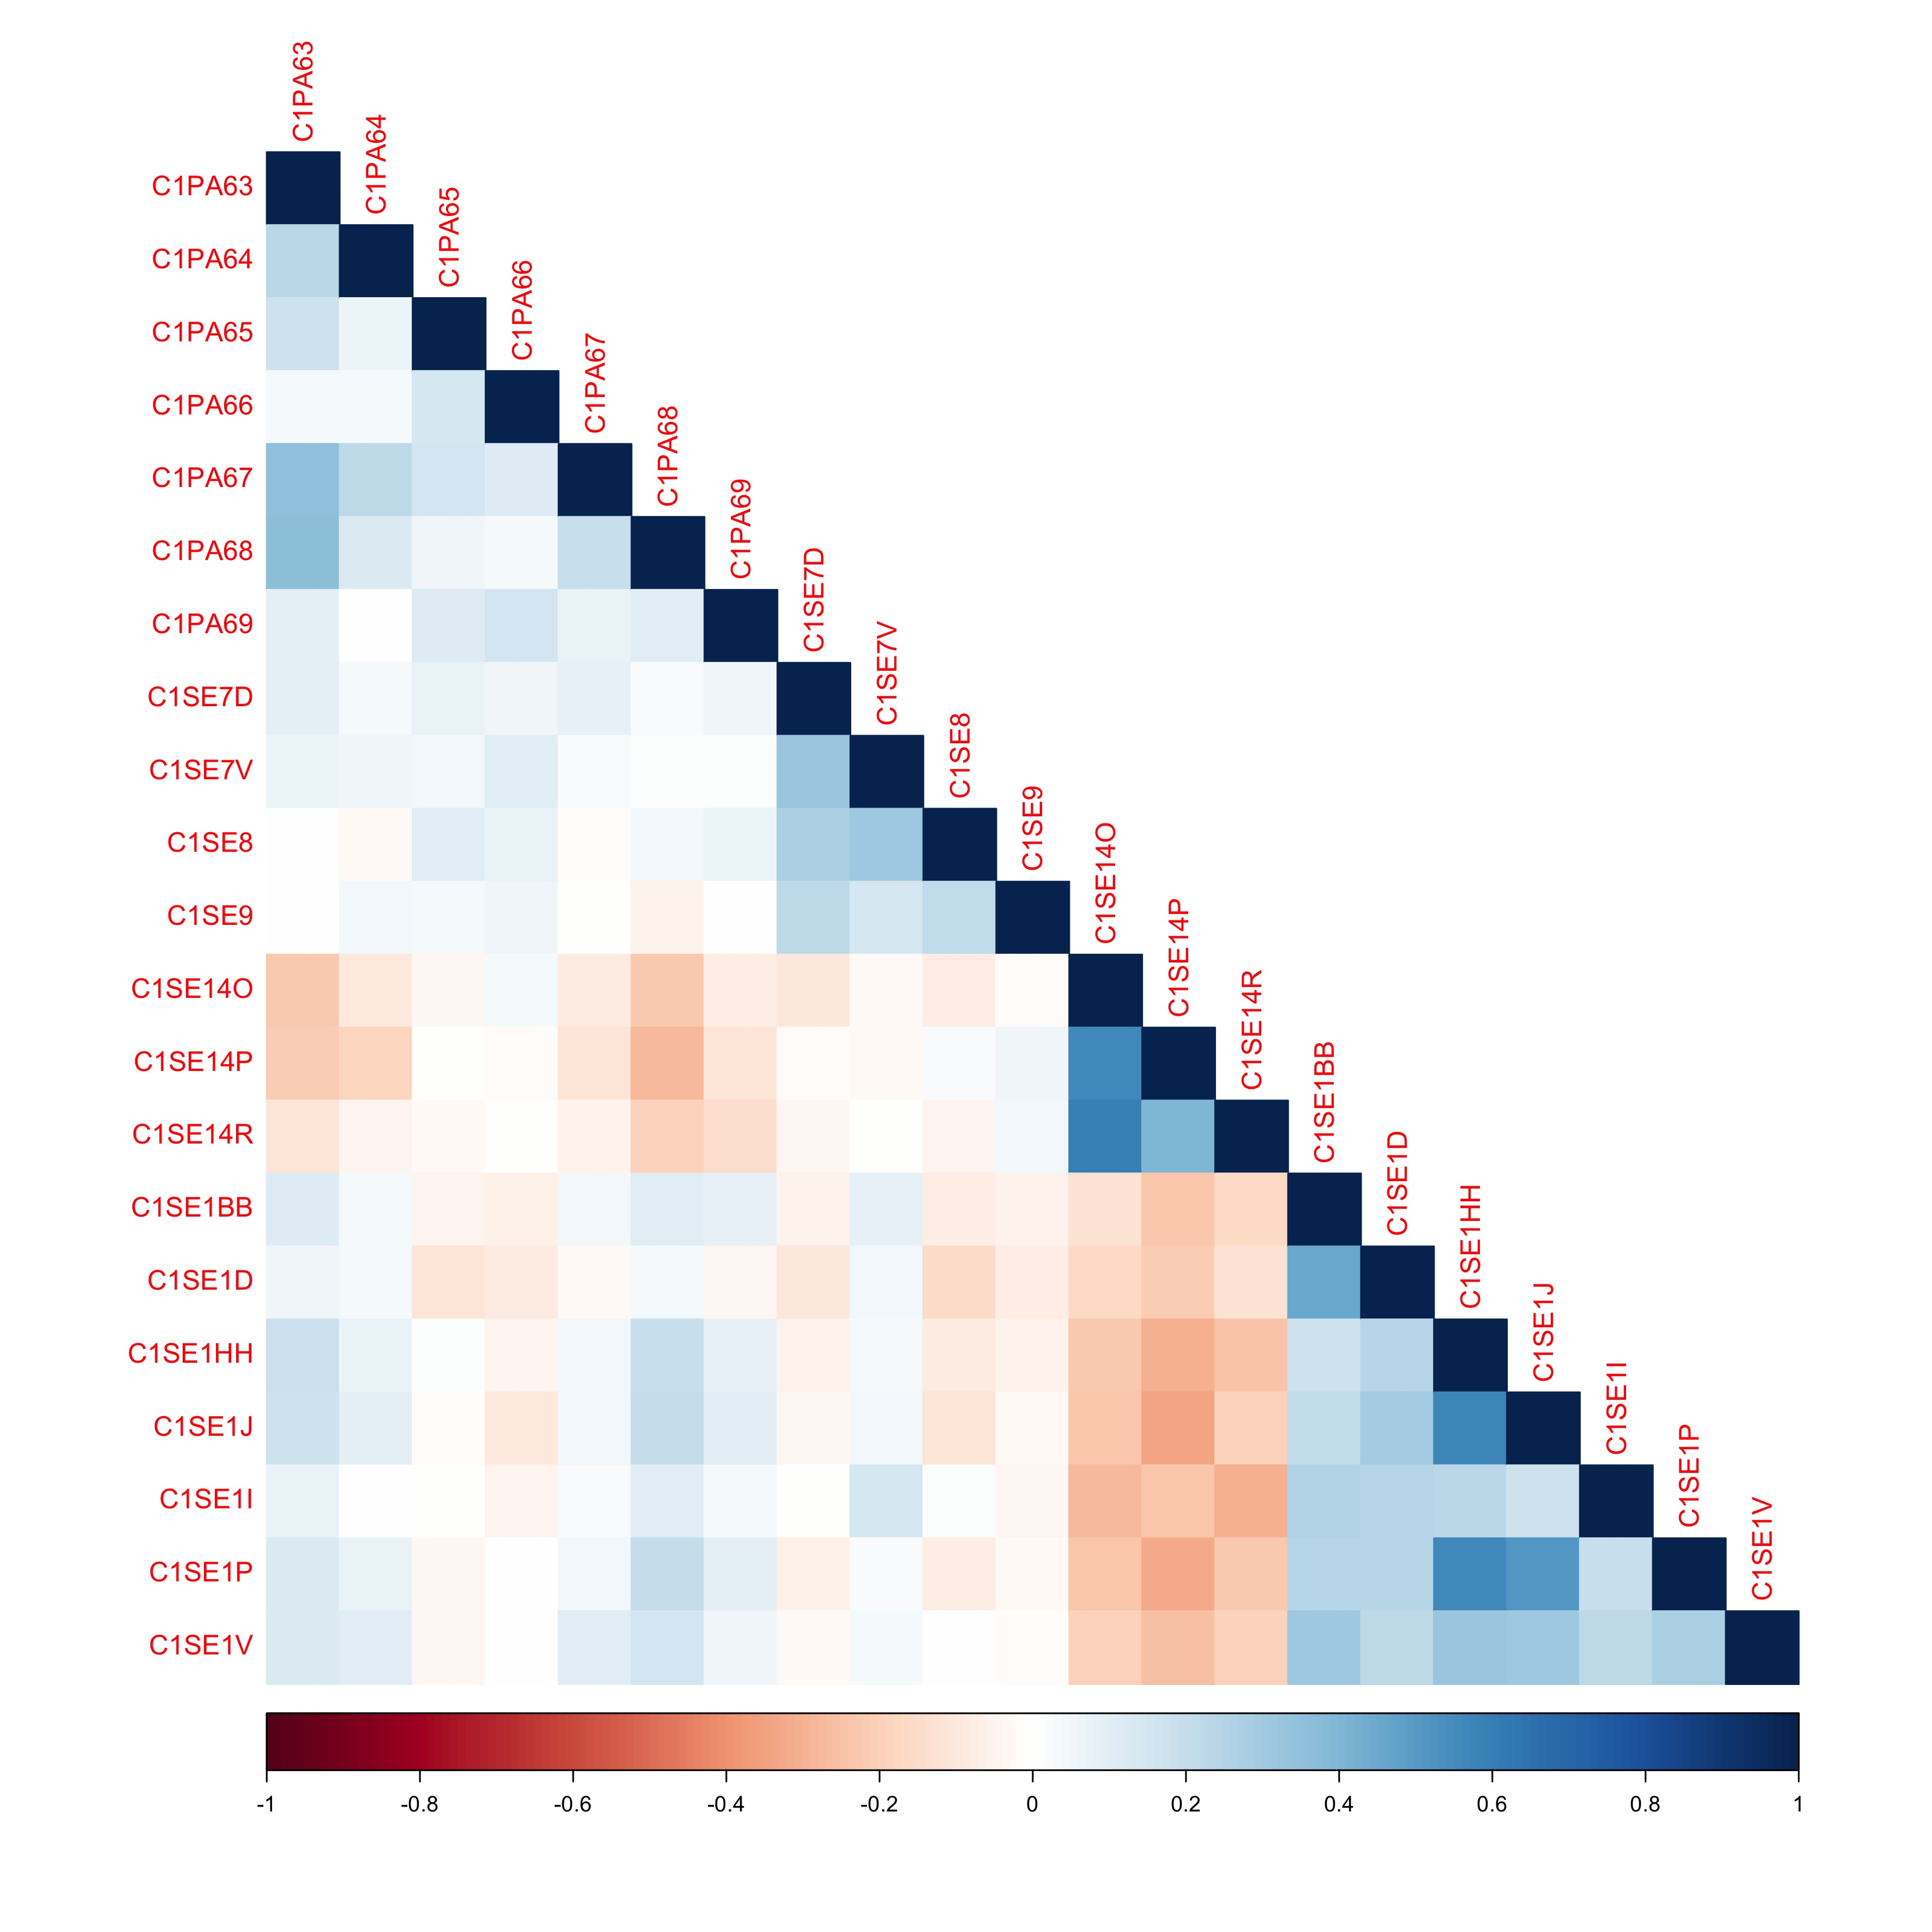
\includegraphics[width=14cm]{../visualizations/corr.png}
\caption{Correlation plot}
\label{fig:corr}
\end{figure}

% Missing data

\FloatBarrier
\pagebreak
\section{The base model}

Next, the base model will be discussed. Based on the work of \textcite{tse2011},
it has been concluded that depression can be explained through the constructs
harm avoidance, self directedness and social functioning. In other words, there
are four latent variables which are related to each other through a structural
model. Harm avoidance and self-directedness have an effect on social functioning.
Social functioning, then, has an effect on depression. Moreover, it was estimated
that there is also a direct effect of self-directedness on depression.
Hence, there should be no direct effect of harm avoidance on depression.

In the previous section it became clear that ordinal variables have been used in
the analysis. Model identification and estimation will therefore be discussed
first. The measurement model indicates how variables are related to their latent
constructs and will be discussed next. Afterwards, a closer look will be taken
at the structural model, since an important aspect in this work is the
relationships between latent variables. Lastly, the model fit will be evaluated
through fit measures and further inspected using modification indices.

\subsection{Model identification and estimation}

% Model identification
First and foremost, model identification and estimation will be discussed.
A structural equation model is said to be identified if every latent variable
has its scale identified and the models degrees of freedom is zero or greater.
To that end, the scale of the first indicator of every latent variable has been
fixed to one. The model contains 92 parameters that should be estimated.
Specifically, there are 17 (21 - 4) loadings, 4 regression parameters, 66
thresholds (more about this later), 1 latent covariance and 4 latent variances.
The degrees of freedom of the model therefore equals 276 (23*24/2) - 92 = 184.
The following assumptions have been made on the equations shown
in \ref{eq:base_model}. The measurement errors $\delta$ are supposed to have an
expected value of 0. It is assumed that they have constant variance across
observations and are mutually uncorrelated. There should be a covariance of zero
between these errors and the latent variables.

\begin{equation}
    \footnotesize
    \label{eq:base_model}
    \begin{cases}
    \textrm{PA63}  & = \lambda_{11} \textrm{depression} + \delta_{11} \\
    \textrm{PA64}  & = \lambda_{12} \textrm{depression} + \delta_{12} \\
    \textrm{PA65}  & = \lambda_{13} \textrm{depression} + \delta_{13} \\
    \textrm{PA66}  & = \lambda_{14} \textrm{depression} + \delta_{14} \\
    \textrm{PA67}  & = \lambda_{15} \textrm{depression} + \delta_{15} \\
    \textrm{PA68}  & = \lambda_{16} \textrm{depression} + \delta_{16} \\
    \textrm{PA69}  & = \lambda_{17} \textrm{depression} + \delta_{17} \\
    \textrm{SE7V}  & = \lambda_{21} \textrm{harm avoidance} + \delta_{21} \\
    \textrm{SE7D}  & = \lambda_{22} \textrm{harm avoidance} + \delta_{22} \\
    \textrm{SE8}   & = \lambda_{23} \textrm{harm avoidance} + \delta_{23} \\
    \textrm{SE9}   & = \lambda_{24} \textrm{harm avoidance} + \delta_{24} \\
    \textrm{SE14O} & = \lambda_{31} \textrm{self-directedness} + \delta_{31} \\
    \textrm{SE14P} & = \lambda_{32} \textrm{self-directedness} + \delta_{32} \\
    \textrm{SE14R} & = \lambda_{33} \textrm{self-directedness} + \delta_{33} \\
    \textrm{SE1BB} & = \lambda_{41} \textrm{social functioning} + \delta_{41} \\
    \textrm{SE1D}  & = \lambda_{42} \textrm{social functioning} + \delta_{42} \\
    \textrm{SE1HH} & = \lambda_{43} \textrm{social functioning} + \delta_{43} \\
    \textrm{SE1J}  & = \lambda_{44} \textrm{social functioning} + \delta_{44} \\
    \textrm{SE1I}  & = \lambda_{45} \textrm{social functioning} + \delta_{45} \\
    \textrm{SE1P}  & = \lambda_{46} \textrm{social functioning} + \delta_{46} \\
    \textrm{SE1V}  & = \lambda_{47} \textrm{social functioning} + \delta_{47} \\
    \textrm{social functioning} & = \beta_1 \textrm{harm avoidance} + \beta_2 \textrm{self-directedness} + \delta_1 \\
    \textrm{depression} & = \beta_3 \textrm{social functioning} + \delta_2 \\
    \textrm{depression} & = \beta_4 \textrm{self-directedness} + \delta_3
    \end{cases}
\end{equation}

\begin{figure}[h!]
\centering
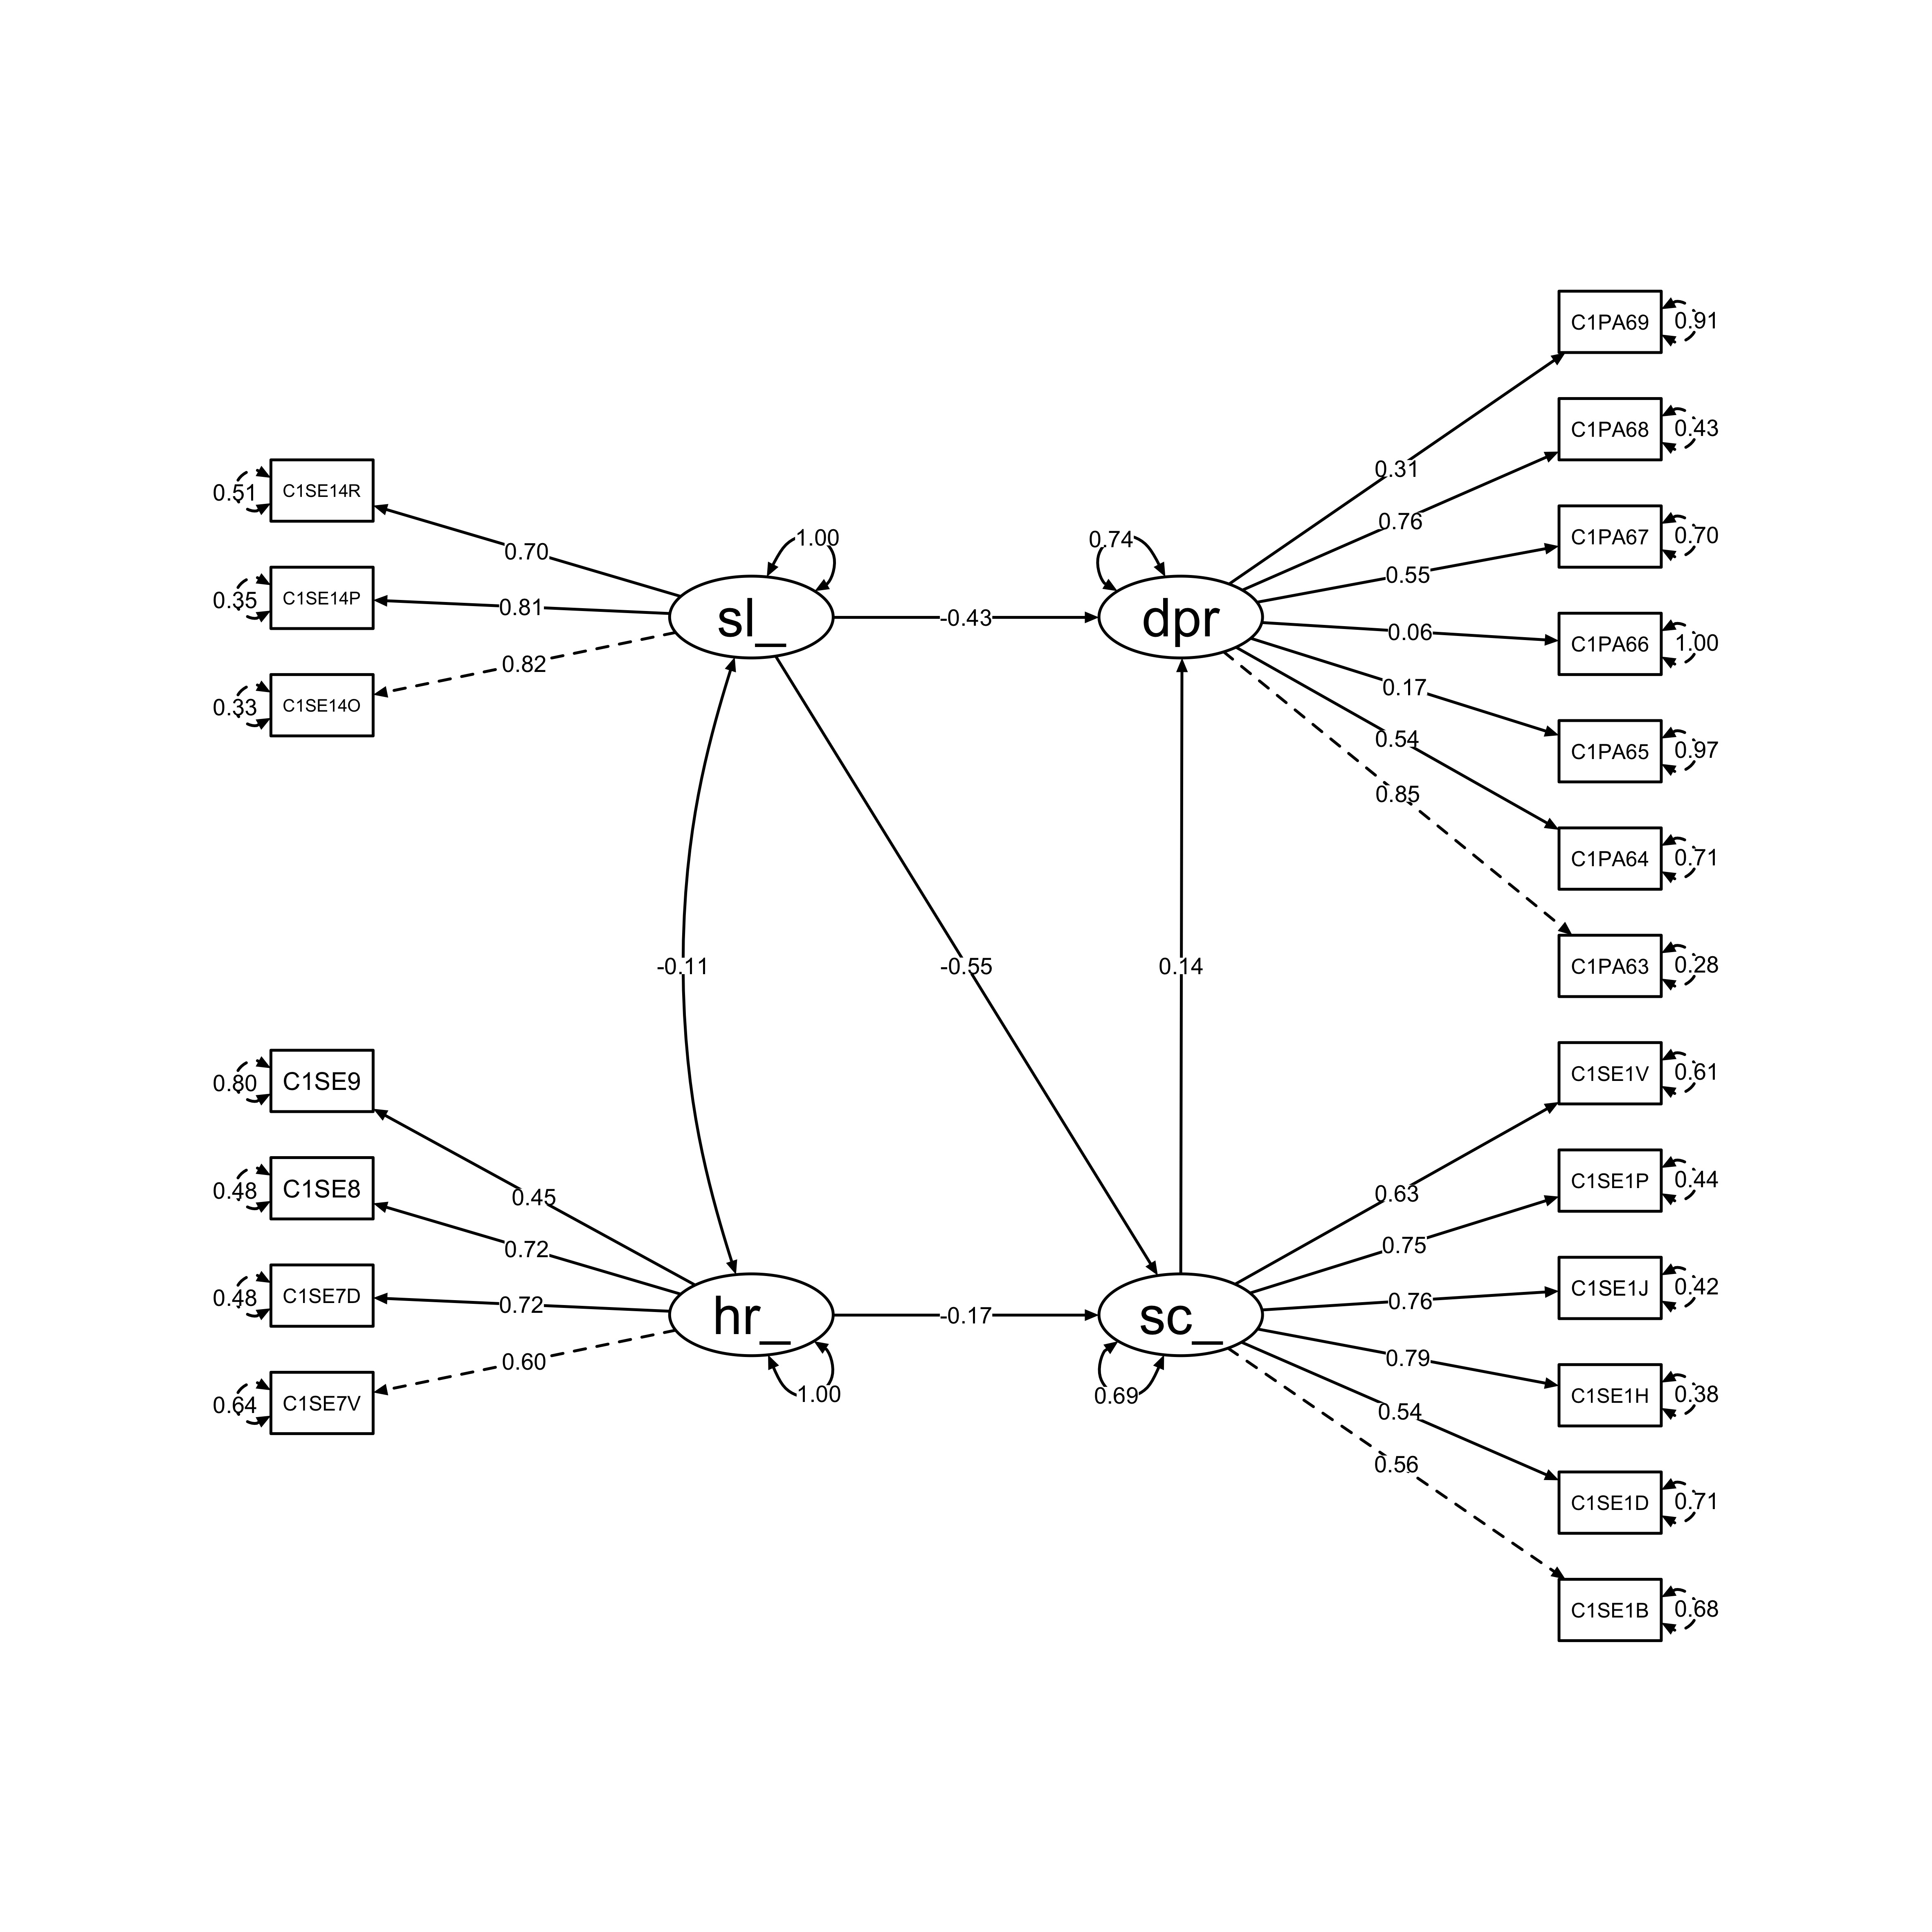
\includegraphics[width=14cm]{../visualizations/base_model.png}
\caption{Summary of the (standardized) base model. hr\_: harm avoidance,
         sl\_: self-directedness, sc\_: social functioning, dpr: depression}
\end{figure}

A considerable problem arises when one considers the assumption of multivariate
normality on the residuals $\delta$. All observed variables are ordinal in nature,
meaning that they are not continuous and should not be treated as such. Their
means and (co)variances have no meaning, since they do not have origins or units
of measurement (\cite{joreskog1994}). The standard maximum likelihood machinery
used in structural equation modeling is therefore not applicable. In this case,
robust maximum likelihood or a least squares approach (unweighted least squares,
diagonally weighted least squares or weighted least squares) can be used
(\cite{yangwallentin2010}). The method of diagonally weighted least squares has
been specifically developed for ordinal data and has been shown to yield better
results when the sample size is not small (\cite{li2016}). It has therefore been
applied here. First, polychoric correlations are estimated. Afterwards, the model
parameters can be estimated. 

First, the polychoric correlations should be estimated. A solution can then be
obtained by assuming that a latent, normal variable $x^*$ is responsible for the
observed ordinal variables $x$. With $x=m$ I mean to say that $x$ belongs to a
category $m$. Generally, the mean and variance if $x^*$ are not identified, since
only ordinal information is available (\cite{simsek2012}). Thresholds are used
to link the latent variable to its observed counterpart:

\begin{equation}
  x = m \:\: \text{if} \:\: \nu_m < x^* < \nu_{m+1} .
\end{equation}

Also, if one assumes $x^*$ is standard normally distributed:

\begin{equation}
  \pi_m = Pr[x=m] = Pr[\nu_m < x^* < \nu_{m+1}] = \int^{\nu_{m+1}}_{\nu_m} \Phi(u)du = \Phi(\nu_{m+1}) - \Phi(\nu_m) .
\end{equation}

In other words, a certain response $m$ from the ordinal variable $x$ is observed,
if the response from its latent variable $x^*$ falls between two thresholds.
Hence, the thresholds are also parameters to be estimated. Second, the model
parameters can be estimated using using a fit function. The ML and DWLS fit
functions are defined as follows:

\begin{align}
  F_{ML} &= \ln |S_{ML}| - \ln |\Sigma| + \text{trace}[(S_{ML})(\Sigma^{-1})] - p \tag{ML fit function} \\
  F_{DWLS} &= [S_{DWLS}-\Sigma]' W^{-1}_D [S_{DWLS}-\Sigma].          \tag{DWLS fit function}
\end{align}

$S_{ML}$ is the covariance or correlation matrix and $S_{DWLS}$ contains the
polychoric correlations. $\Sigma$ is the reproduced covariance or correlation
matrix and depends on the models parameters. $W_D^{-1}$ is a diagonal weight
matrix, which are inversely proportional to the variances of the polychoric
correlations (\cite{yangwallentin2010}). We can therefore conclude that the
DWLS fit function is a weighted least squares approach.

\begin{minipage}{\linewidth}
\begin{lstlisting}
base.model <- "
    # measurement
    depression =~ C1PA63 + C1PA64 + C1PA65 + C1PA66 + C1PA67 + C1PA68 + C1PA69
    harm_avoidance =~ C1SE7V + C1SE7D + C1SE8 + C1SE9
    self_directedness =~ C1SE14O + C1SE14P + C1SE14R
    social_functioning =~ C1SE1BB + C1SE1D + C1SE1HH + C1SE1J + C1SE1I + C1SE1P + C1SE1V

    # structural
    social_functioning~harm_avoidance+self_directedness
    depression~social_functioning
    depression~self_directedness
"

base.fit <- cfa(base.model, data=data, ordered=TRUE)
summary(base.fit, standardized=TRUE, fit.measures=TRUE)
modindices(base.fit, sort=TRUE, maximum.number=20)

jpeg(file="visualizations/base_model.png", width=50, height=50, units="cm", res=400)
semPaths(base.fit, what="diagram", whatLabels="stand", layout="tree2", rotation=2,
         sizeMan=5, sizeMan2=3, sizeLat=10, sizeLat2=4, intercepts=FALSE,
         edge.color="black", thresholds=FALSE, label.scale=TRUE, asize=1.5,
         edge.label.cex=0.5, label.cex=1)
dev.off()
\end{lstlisting}
\end{minipage}

\FloatBarrier
\subsection{Measurement model}

% Measurement model
% More interpretation of loadings here
Second, we will take a closer look at the measurement model, which indicates
how the variables relate to their latent constructs. The factor loading can be
interpreted as the regression slope for predicting the indicator from the latent
variable (\cite{brown2015}). The standardized loading is often more interesting,
since it can then be interpreted as a correlation and one does not need to worry
about the scale of the variables. By squaring the standardized loading the
communality can be obtained, which indicates the proportion of the variance in
the indicator that is explained by the latent variable. The residual variance
then indicates the proportion of the variance that is not explained by the latent
factor. Although there are no hard rules, a popular cut-off value for the
communality appears to be 0.5 (\cite{hair2010}). Based on my observation,
communalities that are a little bit lower are also acceptable, as long as there
is a good theoretical justification for the relationship between the factor and
indicator. The standardized loading should then be larger than 0.7, which means
that the indicator does a good job at reflecting the latent construct.

\begin{table}[h!]
\captionsetup{singlelinecheck=off}
\caption{Measurement model}
\label{tab:measurement_base}
\scalebox{0.8}{
\begin{tabular}{|l|l|l|l|l|l|l|l|}
\hline
\textbf{Variable}                 & \textbf{Loading} & \textbf{Standard error} & \textbf{z-value} & \textbf{p-value}     & \textbf{St. loading}    & \textbf{Communality} & \textbf{Unique var.}   \\ \hline
PA63 \hfill ($\lambda_{11}$)      & 1.000            &                         &                    &                    & 0.847                   &  0.718               & 0.275 \hfill ($\delta_{11}$)  \\ \hline
PA64 \hfill ($\lambda_{12}$)      & 0.646            & 0.108                   &  5.974             & \textless 0.001    & 0.548                   &  0.300               & 0.700 \hfill ($\delta_{12}$)  \\ \hline
PA65 \hfill ($\lambda_{13}$)      & 0.194            & 0.082                   &  2.384             & 0.017              & 0.165                   &  0.027               & 0.973 \hfill ($\delta_{13}$)  \\ \hline
PA66 \hfill ($\lambda_{14}$)      & 0.068            & 0.085                   &  0.806             & 0.420              & 0.058                   &  0.003               & 0.997 \hfill ($\delta_{14}$)  \\ \hline
PA67 \hfill ($\lambda_{15}$)      & 0.657            & 0.096                   &  6.810             & \textless 0.001    & 0.556                   &  0.309               & 0.691 \hfill ($\delta_{15}$)  \\ \hline
PA68 \hfill ($\lambda_{16}$)      & 0.896            & 0.108                   &  8.321             & \textless 0.001    & 0.760                   &  0.578               & 0.422 \hfill ($\delta_{16}$)  \\ \hline
PA69 \hfill ($\lambda_{17}$)      & 0.357            & 0.088                   &  4.076             & \textless 0.001    & 0.303                   &  0.092               & 0.908 \hfill ($\delta_{17}$)  \\ \hline
%                                                                                                               
SE7V \hfill ($\lambda_{21}$)      & 1.000            &                         &                    &                    & 0.604                   &  0.365               & 0.635 \hfill ($\delta_{21}$)  \\ \hline
SE7D \hfill ($\lambda_{22}$)      & 1.186            & 0.153                   &  7.754             & \textless 0.001    & 0.716                   &  0.513               & 0.487 \hfill ($\delta_{22}$)  \\ \hline
SE8  \hfill ($\lambda_{23}$)      & 1.203            & 0.158                   &  7.600             & \textless 0.001    & 0.726                   &  0.527               & 0.473 \hfill ($\delta_{23}$)  \\ \hline
SE9  \hfill ($\lambda_{24}$)      & 0.733            & 0.116                   &  6.322             & \textless 0.001    & 0.442                   &  0.195               & 0.795 \hfill ($\delta_{24}$)  \\ \hline
%                                                                                                                               
SE14O  \hfill ($\lambda_{31}$)    & 1.000            &                         &                    &                    & 0.817                   &  0.667               & 0.333 \hfill ($\delta_{31}$)  \\ \hline
SE14P  \hfill ($\lambda_{32}$)    & 0.984            & 0.048                   & 20.3655            & \textless 0.001    & 0.805                   &  0.648               & 0.352 \hfill ($\delta_{32}$)  \\ \hline
SE14R  \hfill ($\lambda_{33}$)    & 0.866            & 0.047                   & 18.5985            & \textless 0.001    & 0.708                   &  0.501               & 0.499 \hfill ($\delta_{33}$)  \\ \hline
%                                                                                                                               
SE1BB \hfill ($\lambda_{41}$)     & 1.000            &                         &                    &                    & 0.563                   &  0.317               & 0.683 \hfill ($\delta_{41}$)  \\ \hline
SE1D  \hfill ($\lambda_{42}$)     & 0.952            & 0.072                   & 13.3028            & \textless 0.001    & 0.536                   &  0.287               & 0.713 \hfill ($\delta_{42}$)  \\ \hline
SE1HH \hfill ($\lambda_{43}$)     & 1.385            & 0.097                   & 14.2430            & \textless 0.001    & 0.779                   &  0.607               & 0.303 \hfill ($\delta_{43}$)  \\ \hline
SE1J  \hfill ($\lambda_{44}$)     & 1.331            & 0.092                   & 14.4760            & \textless 0.001    & 0.749                   &  0.561               & 0.484 \hfill ($\delta_{44}$)  \\ \hline
SE1I  \hfill ($\lambda_{45}$)     & 0.843            & 0.079                   & 10.6372            & \textless 0.001    & 0.474                   &  0.225               & 0.775 \hfill ($\delta_{45}$)  \\ \hline
SE1P  \hfill ($\lambda_{46}$)     & 1.303            & 0.085                   & 15.2614            & \textless 0.001    & 0.733                   &  0.537               & 0.463 \hfill ($\delta_{46}$)  \\ \hline
SE1V  \hfill ($\lambda_{47}$)     & 1.117            & 0.091                   & 12.2490            & \textless 0.001    & 0.629                   &  0.396               & 0.604 \hfill ($\delta_{47}$)  \\ \hline
\end{tabular}                                                                                                                                           
}
\end{table}
 
Inspecting Table \ref{tab:measurement_base}, it is evident to see that some
indicators have a low communality.
First, the variables PA64, PA65, PA66, PA67 and PA69 load on the latent variable
depression and have a unique variance that is too high. The indicators PA64, PA65
and PA66 assess feeling low on energy, a loss of appetite and trouble falling
asleep. PA66 and PA67 evaluate trouble falling asleep and concentrating. Using
PA69 it was asked whether the participant often thinks about death. A simple way
to improve the model fit may be to reduce the number of variables that load on
depression. However, this action would lead to a decline of the theoretical
support and validity of the model as well (\cite{hair2010}). Since these variables
were specifically designed by the authors of the dataset to measure depression I
have decided against doing so.

Next, the harm avoidance construct, which measures whether a behaviour is done to
avoid novelty and punishment, plays a central role in the model. It is measured
using four indicators: SE7V, SE7D, SE8 and SE9. Unfortunately, we have to again
conclude that some of the indicators have a low communality.
On the one hand, SE7V evaluates whether the participant believes it could be fun
to experience an earthquake. On the other hand, through SE9 the respondent has
to choose between a harmful and a safe situation. These variables have a
communality of 0.379 and 0.201, respectively. Since these variables have been
specifically designed by the authors of the dataset I will also not be deleting
them from the model.

Third, self-directedness has been described as a form of self-determination and
ability to regulate behaviour to suit goals and values (\cite{tse2011}). The
variables that load on this construct evaluate whether the respondent likes to
make plans for the future, knows what to want out of life and finding it helpful
to set goals for the near future. The standardized loadings are high
(0.817, 0.805 and 0.708) and indicate a high correlation between the
indicators and latent variable.

Lastly, we can observe that some of the indicators that share a loading on social
functioning have a low communality. Specifically, the variables SE1D and SE1I
are problematic cases. Using SE1D the respondent has to answer whether he or she
believes that other people see him or her as loving and affectionate. SE1I
evaluates whether the participant thinks that it is important to have new
experiences that challenge how you think about yourself and the world.

\FloatBarrier
\subsection{Structural model}

% Structural model
Third, the structural model is of great interest in this work, since it allows us
to make conclusions about the relationships between the latent constructs.
First, we may consider the direct effect of harm avoidance ($\beta_1$) and
self-directedness ($\beta_2$) on social functioning. Both parameters estimates
are significant and indicate a positive relationship with social functioning.
One the one hand, for one standardized unit increase in harm avoidance, it is
estimated that there will be a 0.141 increase in social functioning. On the
other hand, the standardized parameter estimate of 0.568 associated with
self-directedness indicates a stronger relationship with social functioning.
Next, following the theory proposed by \cite{tse2011}, we may expect there to be
a significant effect of social functioning on depression. The results indicate 
that there is a negative pattern between the two in the sample, but this can not
be estimated to the population.
Lastly, the standardized direct effect of self-directedness on depression is
-0.425. This highly significant (p<0.001) effect indicates that an increase of
one standard deviation in self-directedness will lead to a decrease in depression
of 0.425.

\begin{table}[h!]
\begin{equation}
\footnotesize
  \begin{cases}
    \textrm{social functioning} & = \beta_1 \textrm{harm avoidance} + \beta_2 \textrm{self-directedness} + \delta_1 \\
    \textrm{depression} & = \beta_3 \textrm{social functioning} + \delta_2 \\
    \textrm{depression} & = \beta_4 \textrm{self-directedness} + \delta_3
    \tag{Structural model}
  \end{cases}
\end{equation}
\captionsetup{singlelinecheck=off}
\caption{Structural model}
\label{tab:base_structural}
\scalebox{0.8}{
\begin{tabular}{|l|l|l|l|l|l|}
\hline
\textbf{Parameter} & \textbf{Coefficient}      & \textbf{Standard error} & \textbf{z-value} & \textbf{p-value} & \textbf{Stand. coefficient} \\ \hline
$\beta_1$        &  0.131 \hfill               & 0.055                   &  2.398           & 0.016            &  0.141                      \\ \hline
$\beta_2$        &  0.403 \hfill               & 0.038                   &  10.614          & \textless 0.001  &  0.568                      \\ \hline
$\beta_3$        & -0.190 \hfill               & 0.109                   & -1.748           & 0.080            & -0.126                      \\ \hline
$\beta_4$        & -0.441 \hfill               & 0.084                   & -5.263           & \textless 0.001  & -0.425                      \\ \hline
\end{tabular}
}
\end{table}

Strongly related to the structural model is the notion of discriminant validity.
Discriminant validity gives an indication that theoretically different constructs
should not be highly intercorrelated. In other words, if two latent variables
are highly correlated they could represent the same construct and they could be
merged into one latent variable to obtain a more parsimonious solution
(\cite{brown2015}). The low and insignificant (p=0.108) standardized covariance
of -0.1 between harm avoidance and self-directedness indicates that there is
little evidence for poor discriminant validity.

\subsection{Goodness of fit}

Fourth, the goodness of fit of the model will be evaluated.
% Goodness of fit
The $\chi^2$ statistic is closely related to the fit of the model and is very
popular in the literature, but it has received some important criticisms. It has
been noted that in many instances the underlying distribution is not $\chi^2$
distributed, which severely limits the interpretability. Moreover, it is
inflated by sample size and it makes the stringent hypothesis that the sample
covariance matrix and reproduced covariance matrix are equal (\cite{brown2015}).
In this illustration, the test statistic of 589.88 is larger than the critical
value of 216.65. Hence, the null hypothesis that this model is equal to a
perfectly fitting model can be rejected and poor model fit is concluded. However,
given the large sample size of 601 this conclusion should not be trusted.

% Absolute fit
Absolute fit indices have therefore been employed. They assess the quality of
the solution without taking into account model parsimony. First, the standardized
root mean square residual (SRMR) can be interpreted as the average standardized
residual covariance (polychoric correlation). It can be calculated using the
following equation, where $p$ is the number of indicators and $\epsilon$ is
the vector of the standardized residual covariances (\cite{shi2020}). In this
illustration a SRMR of 0.081 was obtained, which indicates borderline poor model
fit as it is just above the target of 0.08.

\begin{equation}
  SRMR = \sqrt{\dfrac{\epsilon \epsilon}{p(p+1)/2}}
\end{equation}

Second, the root mean square error of approximation (RMSEA) takes into
account the error of approximation in the population. The RMSEA takes values
between zero and one and the fit of the model is acceptable if it falls under 0.05.
A RMSEA of 0.065 has been obtained.

I have noticed that sometimes $N$ or $N-1$ is used in the literature. For
consistency I have chosen to use $N$.

\begin{equation}
  RMSEA = \sqrt{\dfrac{\chi^2 - df}{N \times df}}
\end{equation}

\begin{equation}
  RMSEA = \sqrt{\dfrac{a (N-1) (\chi^2 - df) + b}{(N-1) df} - \dfrac{1}{N-1}}
\end{equation}

% Comparative fit
CFI and TLI are two comparative fit indices that will be evaluated as well.
This group of statistics is called comparative, since they make a comparison
between a restricted null model and an alternative model supplied by
the model-builder (\cite{brown2015}). The comparative fit index (CFI) and
Tucker-Lewis index (TLI) have been shown below. Both measures have a range of
possible values from zero to one and make a correction for complexity through
the degrees of freedom. Values that are close to one imply a good model fit.
Generally, 0.9 is taken as a target value. In this illustration the CFI and
TLI are, respectively, 0.938 and 0.93. To sum up, the fit of this model is
borderline good or bad, depending on which fit measures are taken into account.

\begin{equation}
    CFI = \dfrac{(\chi^2 - df)_{null} - (\chi^2 - df)_{alternative}}{(\chi^2 - df)_{null}}
\end{equation}

\begin{equation}
    TLI = \dfrac{(\chi^2 / df)_{null} - (\chi^2 / df)_{null}}{(\chi^2 / df)_{null}}
\end{equation}

\begin{table}[h!]
\captionsetup{singlelinecheck=off}
\caption{Test statistics}
\scalebox{0.8}{
\begin{tabular}{|l|l|l|}
\hline
\textbf{Statistic} & \textbf{Value} & \textbf{Target}   \\ \hline
$\chi^2$           & 589.88         & < 216.65          \\ \hline
CFI                & 0.947          & > 0.9             \\ \hline
TLI                & 0.940          & > 0.9             \\ \hline
RMSEA              & 0.060          & < 0.05            \\ \hline
SRMR               & 0.081          & < 0.08            \\ \hline
\end{tabular}
}
\end{table}

\begin{table}[h!]
\captionsetup{singlelinecheck=off}
\caption{10 highest modification indices of base model}
\label{tab:base_modification}
\scalebox{0.8}{
\begin{tabular}{|l|l|l|l|l|l|}
\hline
\textbf{Left hand side} & \textbf{Operation} & \textbf{Right hand side} & \textbf{\begin{tabular}[c]{@{}l@{}}Modification\\ index\end{tabular}} & \textbf{\begin{tabular}[c]{@{}l@{}}Expected parameter\\ change\end{tabular}} & \textbf{\begin{tabular}[c]{@{}l@{}}Stand. expected\\ parameter change\end{tabular}} \\ \hline
C1SE1BB                 & correlation        & C1SE1D                   & 88.582                                                                & 0.322                                                                        & 0.462                                                                               \\ \hline
self-directedness       & loading            & C1SE1I                   & 49.044                                                                & 0.396                                                                        & 0.323                                                                               \\ \hline
C1SE14O                 & correlation        & C1SE14R                  & 35.183                                                                & 0.273                                                                        & 0.670                                                                               \\ \hline
C1SE1BB                 & correlation        & C1SE1HH                  & 32.460                                                                & -0.278                                                                       & -0.538                                                                              \\ \hline
social functioning     & loading            & C1PA65                   & 32.008                                                                & 0.426                                                                        & 0.240                                                                               \\ \hline
social functioning     & loading            & C1SE14P                  & 27.723                                                                & 0.516                                                                        & 0.290                                                                               \\ \hline
C1SE1HH                 & correlation        & C1SE1J                   & 26.321                                                                & 0.188                                                                        & 0.452                                                                               \\ \hline
social functioning     & loading            & C1SE7V                   & 26.143                                                                & -0.283                                                                       & -0.159                                                                              \\ \hline
C1SE14R                 & correlation        & C1SE1I                   & 25.824                                                                & 0.197                                                                        & 0.317                                                                               \\ \hline
social functioning     & correlation        & C1PA66                   & 24.609                                                                & 0.388                                                                        & 0.219                                                                               \\ \hline
\end{tabular}
}
\end{table}

The modification indices can be used to further investigate sources of model misfit.
They can be calculated for each fixed and constrained parameter in the model and indicate how much the model $\chi^2$ would drop if the parameter was freely estimated.
A good fitting model should then also produce modification indices that are small in magnitude.
A modification index that is greater than 3.84 indicates that the model fit can be significantly improved if the parameter is freely estimated (\cite{brown2015}).
Unfortunately, the summary shown in Table \ref{tab:base_modification} indicates that there are various sources of badness of fit in the model.

First, there are some modification indices associated with the measurement model that can provide insight in sources of the badness of fit.
% 1SE1BB <=> SE1D: YES
It is estimated that the model fit can be improved dramatically by allowing a correlated error term between the variables 1SE1BB and SE1D, which load on social functioning.
On the one hand, SE1BB assesses whether the respondent believes other people would describe him/her as a giving person.
On the other hand, SE1D evaluates whether the respondent believes other people see him/her as loving and affectionate.
Personally, I believe that it is very plausible that these two variables are related to one another.
A correlation between these variables will therefore be allowed in the improved model.

% 1SE14O <=> 1SE14R: NO
Next, the modification indices indicate that the model fit would improve dramatically should a correlated error term be allowed between the self-directedness variables 1SE14O and 1SE14R.
In 1SE14O and 1SE14R it is asked whether the respondent likes to make plans for the future and knows what to want out of life, respectively. 
Since I cannot see how these questions are directly related to each other, I will not allow a correlated error term between them in the improved model.

% 1SE1HH <=>1SE1J: YES
Another area where the model could be improved has to do with the variables 1SE1HH and 1SE1J, which load on social functioning.
On the one hand, in 1SE1HH it is asked whether the participant has experienced many warm and trusting relationships.
On the other hand, for 1SE1J it is asked whether he or she has difficulty maintaining close relationships.
Clearly, if one has difficulty maintaining close relationships, one would also not have experienced many warm and trusting relationships.
A correlated error term will therefore be allowed between these variables in the improved model.

% 1SE1HH <=> 1SE1BB: YES
It is estimated that the model fit can be improved drastically should a correlation error term be allowed between the variables 1SE1BB and 1SE1HH.
Both variables have a loading on social functioning.
1SE1HH indicates whether the respondent has experienced many warm and trusting relationships.
1SE1BB assesses whether the respondent believes he or she would be described by others as a giving person, willing to share his or her time.
Personally, I cannot see how both variables are directly related to each other.
A correlated error term will therefore not be allowed.

% 1SE1HH <=> 1SE1P: YES
Additionally, the modification indices indicate that the variables 1SE1HH and 1SE1P should share a correlation.
1SE1P indicates whether the respondent often feels lonely because he or she has few close friends with whom to share concerns.
Since 1SE1HH assesses whether he or she has experienced many warm and trusting relationships, I believe such a correlation should be allowed.

Second, some modification indices indicate that the structural model is not plausible.
The second and third largest modification specify that there should be a direct relationship between depression and self-directedness.
Moreover, a drop of 27 in $\chi^2$ can be achieved by allowing a direct relationship between depression and harm avoidance through a regression.


\FloatBarrier
\pagebreak
\section{Expanding the base model}

\FloatBarrier
\pagebreak
\section{Conclusion}

\end{document}
